\documentclass[11pt]{article}
\usepackage[utf8]{inputenc}
\usepackage{polski}
\usepackage{graphicx}
\usepackage{array}
\usepackage{paralist}
\usepackage{verbatim}
\usepackage{subfig}
\usepackage{amsmath}
\usepackage{float}
\usepackage{amsthm}
\usepackage{amssymb}
\usepackage{pdfpages}
\usepackage{amsfonts}
\usepackage{tikz}
\usepackage[linguistics]{forest}
\usetikzlibrary{shapes,backgrounds}
\usepackage[margin=1in]{geometry}
\setlength\parindent{0pt}
\theoremstyle{definition}
\newtheorem{zadanie}{Zadanie}
\numberwithin{zadanie}{section}
\renewcommand*{\proofname}{Rozwiązanie}
\maxdeadcycles=1000
\extrafloats{1000}
\title{Rachunek prawdopodobieństwa i statystyka}
\author{Igor Nowicki}
\begin{document}
\maketitle
\tableofcontents

\section{Drugie kolokwium}
\subsection{Ściąga}

\begin{itemize}
    \item Dystrybuanta: $F(X) = \int_\Omega f(x)\text dx$,
    \item wartość oczekiwana: $EX = \int_\Omega x\cdot f(x)\text dx$,
    \item wariancja: $\sigma^2 = \int_\Omega(x-EX)\cdot f(x)\text dx$,
    \item odchylenie standardowe: $\sigma = \sqrt{\sigma^2} = \sqrt{\int_\Omega(x-EX)\cdot f(x)\text dx}$.
    \item Schemat Bernoulliego - prawdopodobieństwo uzyskania $k$ sukcesów w $n$ próbach: $P_n(k) = \binom nk p^k(1-p)^{n-k},$
    \item Przybliżenie Poissona (dla $np^2\ll 1$): $f(k,\lambda) = \frac{\lambda^ke^{-\lambda}}{k!}$.
    \item Rozkład geometryczny, w którym zakładamy że proces odniesie sukces dokładnie w $k$-tej próbie, gdzie $k$ jest liczbą naturalną, dodatnią: $P(X=k) = (1-p)^{k-1}p$.
    \item Wartość oczekiwana dla rozkładu geometrycznego: $EX = \frac1p,$
    \item Wariancja dla rozkładu geometrycznego:  $\sigma^2 = \text{Var}(X) = \frac{1-p}{p^2}$
    \item Odchylenie standardowe dla rozkładu geometrycznego:  $\sigma = \sqrt{\text{Var}(X)} = \sqrt{\frac{1-p}{p^2}}$
    \item Rozkład hipergeometryczny, w którym ze zbioru $N$ elementów w którym jest $R$ elementów wyróżnionych pobieramy losowo $n$ elementów i sprawdzamy jaka jest szansa by $k$ elementów było wyróżnionych:
          $P(X=k)=HG(N,R,n)=\frac{\binom Rk\binom{N-n}{R-k}}{\binom NR} = \frac{\binom nk\binom{N-n}{R-k}}{\binom NR}$.
    \item Gęstość prawdopodobieństwa dla rozkładu wykładniczego to $f(x)=\lambda e^{-\lambda x},$ gdzie $x$ oznacza odstęp czasu między awariami.
    \item Dystrybuanta dla rozkładuw wykładniczego to: $F(x) = 1-e^{-\lambda x}.$
    \item Średni czas odstępu między awariami to: $\bar x_{\text{śr}} = \int_0^\infty x\cdot \lambda e^{-\lambda x}\text dx$.
    \item Rozkład normalny: $f(x, \mu, \sigma) = \frac1{\sigma\sqrt{2\pi}}\exp(-\frac{(x-\mu)^2}{2\sigma^2})$.
    \item Przekształcenia dla innych wartości średniej i wariancji $(\mu, \sigma^2)$: $u=\frac{x-\mu}{\sigma}$.

\end{itemize}

\newpage
\subsection{Zmienne dyskretne}

\begin{zadanie}
    Prawdopodobieństwa uzyskania poszczególnych ocen z egzaminu z RPS są następujące:

    \begin{center}
        \begin{tabular}{ |c|c|c|c|c| }
            \hline
            $x_i$ & 2    & 3    & 4 & 5 \\
            \hline
            $p_i$ & 0.15 & 0.55 & a & b \\
            \hline
        \end{tabular}
    \end{center}

    Wiadomo, że prawdopodobieństwo uzyskania piątki jest dwa razy większe niż uzyskania czwórki.

    \begin{enumerate}[a)]
        \item Wyznacz wartości stałych a i b tak, aby powyższa tabelka określała rozkład prawdopodobieństwa zmiennej losowej opisujacej możliwą do uzyskania ocenę z egzaminu.
        \item Sporzadź wykres funkcji prawdopodobieństwa.
        \item Wyznacz dystrybuantę tej zmiennej losowej i sporządź jej wykres.
        \item Wyznacz i zinterpretuj prawdopodobieństwa: $P (X > 3)$, $P (X \geq 3)$, $P (3 < X \leq 4)$.
        \item Wyznacz wartość oczekiwaną, wariancję oraz odchylenie standardowe zmiennej losowej.
    \end{enumerate}
\end{zadanie}
\begin{proof}

    \begin{enumerate}[a)]
        \item  Wyznacz wartości stałych a i b tak, aby powyższa tabelka określała rozkład prawdopodobieństwa zmiennej losowej opisujacej możliwą do uzyskania ocenę z egzaminu.

              Wiadomo, że szansa uzyskania jakiejkolwiek oceny powinna być równa $1$. Razem z informacją, że $b=2a$, mamy równanie:
              \begin{align*}
                  0.15+0.55+a+b & = 1,   \\
                  0.7+a+2a      & = 1,   \\
                  3a            & = 0.3, \\
                  a             & = 0.1, \\
                  b             & = 0.2.
              \end{align*}

              Uzupełniona tabelka prawdopodobieństw wygląda następująco:

              \begin{center}
                  \begin{tabular}{ |c|c|c|c|c| }
                      \hline
                      $x_i$ & 2    & 3    & 4   & 5   \\
                      \hline
                      $p_i$ & 0.15 & 0.55 & 0.1 & 0.2 \\
                      \hline
                  \end{tabular}
              \end{center}

        \item Sporządź wykres funkcji prawdopodobieństwa.

              \begin{figure}[H]
                  \centering
                  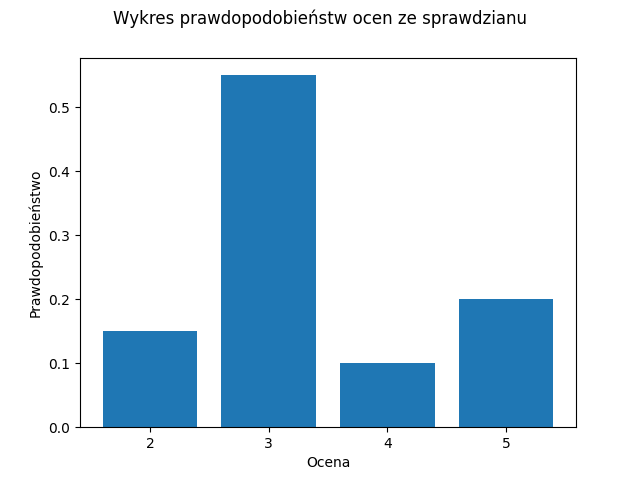
\includegraphics[width=0.5\linewidth]{oceny.png}
              \end{figure}

        \item Wyznacz dystrybuantę tej zmiennej losowej i sporządź jej wykres.

              Dystrybuantę $F$ definiuje się następująco:

              $$F(t) = \mathbb F((-\infty, t]).$$

              Dla rozkładu dyskretnego możemy zastosować następujący wzór:

              $$F(x_k) = \sum_{i=0}^{k} p_i.$$

              W ten sposób możemy stworzyć nową tabelę dla dystrybuanty ocen.

              \begin{center}
                  \begin{tabular}{ |c|c|c|c|c| }
                      \hline
                      $x_i$    & 2    & 3   & 4   & 5 \\
                      \hline
                      $F(x_i)$ & 0.15 & 0.7 & 0.8 & 1 \\
                      \hline
                  \end{tabular}
              \end{center}

              Wykres dystrybuanty:

              \begin{figure}[H]
                  \centering
                  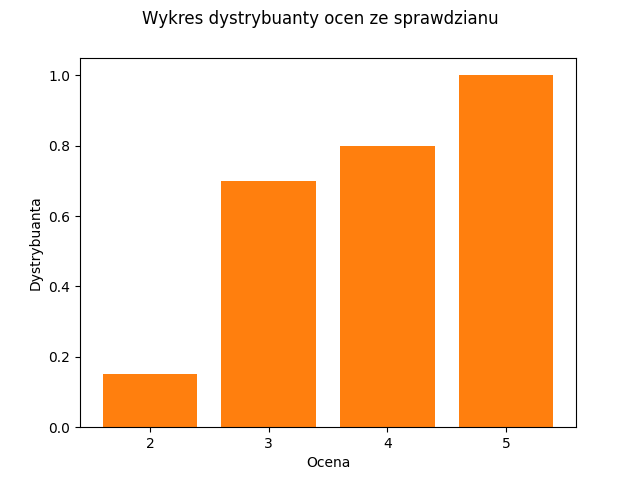
\includegraphics[width=0.5\linewidth]{oceny-dyst.png}
              \end{figure}

        \item Wyznacz i zinterpretuj prawdopodobieństwa:
              \begin{itemize}
                  \item $P (X > 3) = \mathbb F(\infty) - \mathbb F(3) = 0.3$ - prawdopodobieństwo otrzymania oceny lepszej niż 3,
                  \item $P (X \geq 3) = \mathbb F(\infty) - \mathbb F(2) = 0.85$ - prawdopodobieństwo zdania egzaminu z oceną pozytywną,
                  \item $P (3 < X \leq 4) = \mathbb F(4) - \mathbb F(3)$ - prawdopodobieństwo zdania egzaminu na 4.
              \end{itemize}
        \item Wyznacz wartość oczekiwaną, wariancję oraz odchylenie standardowe zmiennej losowej.

              \begin{itemize}
                  \item Wartość oczekiwana: $\mathbb E(X)= \sum_i x_ip_i = 2\cdot0.15+3\cdot0.55+4\cdot0.1+5\cdot0.2 = 3.35$,
                  \item Wariancja: $\sigma^2 = \sum_i(x_i-\bar x)^2\cdot p_i= 0.9275$,
                  \item Odchylenie standardowe: $\sigma = \sqrt{\sigma^2} = \sqrt{0.9275} \approx 0.963$.
              \end{itemize}

    \end{enumerate}
\end{proof}

\begin{zadanie}

    Dystrybuanta pewnej dyskretnej zmiennej losowej dana jest wzorem

    \begin{align*}
                       & 0   & \text{ dla } x \in (-\infty, -2) \\
        F (x)  =\qquad & 0.4 & \text{ dla } x \in [-2, 3)       \\
                       & 0.5 & \text{ dla } x \in [3, 5)        \\
                       & 1   & \text{ dla } x \in [5, +\infty)
    \end{align*}

    Wyznacz funkcję prawdopodobieństwa tej zmiennej. Oblicz:
    \begin{enumerate}[a)]
        \item $P (X \leq -2),$
        \item $P (X < 3),$
        \item $P (X \geq 3),$
        \item $P (-2 \leq X \leq 5),$
        \item $P (-2 \leq X < 5).$
    \end{enumerate}
\end{zadanie}
\begin{proof}
    Funkcja prawdopodobieństwa zmiennej:

    \begin{center}
        \begin{tabular}{ |c|c|c|c| }
            \hline
            $x_i$ & -2  & 3   & 5   \\
            \hline
            $p_i$ & 0.4 & 0.1 & 0.5 \\
            \hline
        \end{tabular}
    \end{center}

    \begin{enumerate}[a)]
        \item $P (X \leq -2) = 0.4$
        \item $P (X < 3) = 0.4,$
        \item $P (X \geq 3) = 0.6,$
        \item $P (-2 \leq X \leq 5) = 1,$
        \item $P (-2 \leq X < 5) = 0.5.$
    \end{enumerate}
\end{proof}

\begin{zadanie}
    Wirus komputerowy próbuje uszkodzić dwa pliki. Pierwszy z nich zostanie uszkodzony z prawdopodobieństwem 0.4.
    Niezależnie od tego, drugi zostanie uszkodzony z prawdopodobieństwem 0.3. Wyznacz rozkład oraz dystrybuantę
    zmiennej losowej X opisujacej możliwą liczbę uszkodzonych plików.
\end{zadanie}
\begin{proof}
    Szansa na uszkodzenie:
    \begin{itemize}
        \item Żadnego pliku: $P((A\cap B)') = 1-\big(P(A)+P(B)-P(A\cap B)\big)  = 0.42$.
        \item Jednego pliku: $P(A\oplus B) = P(A)+P(B)-2P(A\cap B)=0.4+0.3-0.24=0.46$.
        \item Obydwu plików: $P(A\cap B) = 0.4\cdot0.3=0.12$.
    \end{itemize}

    Rozkład prawdopodobieństw i dystrybuanta:

    \begin{center}
        \begin{tabular}{ |c|c|c|c| }
            \hline
            $x_i$    & 0    & 1    & 2    \\
            \hline
            $p_i$    & 0.42 & 0.46 & 0.12 \\
            \hline
            $F(x_i)$ & 0.42 & 0.88 & 1    \\
            \hline
        \end{tabular}
    \end{center}


\end{proof}

Do rozwiązania poniższych zadań potrzebujemy \textbf{schematu Bernoulliego} na prawdopodobieństwo uzyskania $k$ sukcesów w $n$ próbach:

$$P_n(k) = \binom nk p^k(1-p)^{n-k},$$

gdzie $p$ jest prawdopodobieństwem sukcesu w jednej próbie.

\begin{zadanie} Oblicz prawdopodobieństwo tego, że rzucajac pięć razy kostką wyrzucimy trzy razy szóstkę.\end{zadanie}

\begin{proof}
    Oblicz prawdopodobieństwo tego, że rzucajac pięć razy kostką wyrzucimy trzy razy szóstkę:
    $$P_5(3) = \binom 53 \Bigg(\frac16\Bigg)^3\Bigg(\frac56\Bigg)^2 \approx 3.215\% $$
\end{proof}

\begin{zadanie}
    Szacuje się, że aż 10\% studentów nie lubi zajęć z RPS. Jakie jest prawdopodobieństwo, że wśród 6 przypadkowo
    napotkanych studentów co najmniej dwóch nie będzie lubiło tego przedmiotu?
\end{zadanie}
\begin{proof}
    Skorzystamy ze znanego skądinąd wzoru na prawdopodobieństwo dopełnienia:

    $$\mathcal P(A') = 1 - \mathcal P(A).$$

    A zatem - prawdopodobieństwo że co najmniej dwóch studentów nie lubi przedmiotu jest dopełnieniem prawdopodobieństwa że co najwyżej jeden student nie lubi przedmiotu. To prawdopodobieństwo można wyrazić jako:

    $$\mathcal P(A') = \mathcal P(A_0)+\mathcal P(A_1) = \binom60\cdot0.1^0\cdot0.9^6+\binom61\cdot0.1^1\cdot0.9^5 = 0.9^6+6\cdot0.1\cdot0.9^5 = 88.57\%.$$

    Zatem szansa że co najmniej dwóch studentów nie będzie lubiło przedmiotu wynosi $\mathcal P(A) = 1-\mathcal P(A') = 1-88.57\%=11.43\%$.

\end{proof}
\begin{zadanie}
    Janek spóźnia się do pracy z prawdopodobieństwem 0.15 każdego dnia. Interesuje nas możliwa liczba dni w tygodniu
    (5 dni roboczych), w których Janek spóźnia się do pracy.
    \begin{enumerate}[a)]
        \item Wyznacz funkcję rozkładu prawdopodobieństwa i dystrybuantę liczby spóźnień w ciagu 5 dni.
        \item Jakie jest prawdopodobieństwo, że w ciagu 5 dni Janek spóźni się co najwyżej raz?
    \end{enumerate}
\end{zadanie}
\begin{proof}

    \begin{enumerate}[a)]
        \item Wyznacz funkcję rozkładu prawdopodobieństwa i dystrybuantę liczby spóźnień w ciagu 5 dni.

              Zastosujemy rozkład Bernoulliego:

              $$\mathcal P_n(k) = \binom nkp^k(1-p)^{n-k},$$

              gdzie $n=5$ to liczba dni w tygodniu (roboczym), a $k$ to liczba dni w których Janek się spóźnił. Zatem:


              \begin{center}
                  \begin{tabular}{ |c|c|c|c|c|c|c| }
                      \hline
                      $k$               & 0       & 1       & 2       & 3       & 4       & 5       \\
                      \hline
                      $\mathcal P_5(k)$ & 44.37\% & 39.15\% & 13.82\% & 2.43\%  & 0.21\%  & 0.001\% \\
                      \hline
                      $\mathcal F(k)$   & 44.37\% & 83.52\% & 97.34\% & 99.78\% & 99.99\% & 100\%   \\
                      \hline
                  \end{tabular}
              \end{center}



        \item Jakie jest prawdopodobieństwo, że w ciagu 5 dni Janek spóźni się co najwyżej raz?

              Szansa że Janek spóźni się najwyżej raz to suma szans że spóźni się zero lub jeden razy - zatem prawdopodobieństwo bedzie równe dystrybuancie $\mathcal F(1)=83.52\%$.

    \end{enumerate}
\end{proof}
\begin{zadanie}
    W statystycznej kontroli jakości partia wyrobów zostaje zaakceptowana jako dobra tylko wtedy, gdy liczba sztuk
    wadliwych w stosunku do liczebności całej partii nie przekracza pewnej z góry określonej wartości. Przypuśćmy, że
    w dużej partii wyrobów jest 20\% sztuk wadliwych. Pobrano próbę liczacą 20 sztuk. Procedura kontrolna przewiduje
    zaakceptowanie partii wyrobów tylko wtedy, gdy nie więcej niż 2 sztuki wśród 20 okażą się wadliwe. Jakie jest
    prawdopodobieństwo, że partia wyrobów nie zostanie zaakceptowana?
\end{zadanie}
\begin{proof}
    Szansa że partia wyrobów nie zostanie zaakceptowana jest dopełnieniem szansy że zostanie zaakceptowana, tj. nie więcej niż dwie sztuki będą wadliwe. Szansa na to że co najwyżej dwie sztuki są wadliwe jest równa dystrybuancie $\mathcal F(2) = p_{20}(0)+p_{20}(1)+p_{20}(2)$. Potrzebujemy obliczyć prawdopodobieństwa $ p_{20}(0), p_{20}(1), p_{20}(2)$ - uzyskujemy je ze wzoru Bernoulliego:

    \begin{align*}
        p_{20}(0) & =\binom{20}{0}\cdot0.2^0\cdot0.8^{20}= 1.15\%,  \\
        p_{20}(1) & =\binom{20}{1}\cdot0.2^1\cdot0.8^{19}= 5.76\%,  \\
        p_{20}(2) & =\binom{20}{2}\cdot0.2^2\cdot0.8^{18}= 13.69\%.
    \end{align*}

    Suma powyższych prawdopodobieństw to $20.6\%$ - jest to szansa że partia zostanie zaakceptowana. Zatem szansa że partia będzie odrzucona wynosi $79.4\%$.

\end{proof}
\begin{zadanie}
    Prawdopodobieństwo trafienia przez strzelca w dziesiatkę jest równe 0.7, a w dziewiątkę - 0.3. Oblicz prawdopodobieństwo, że strzelec zdobędzie przy trzech strzałach co najmniej 29 punktów.
\end{zadanie}
\begin{proof}
    Aby strzelec uzyskał co najmniej 29 punktów w trzech strzałach, musi spudłować (tj. trafić w dziewiątkę) co najwyżej raz. Prawdopodobieństwa strzałów obliczamy z rozkładu Bernoulliego:

    \begin{align*}
        p_{3}(0) & =\binom{3}{0}\cdot0.7^3\cdot0.3^{0}= 34.3\%, \\
        p_{3}(1) & =\binom{3}{1}\cdot0.7^1\cdot0.3^{2}= 44.1\%.
    \end{align*}

    Szansa że strzelec spudłuje co najwyżej raz jest równa dystrybuancie $\mathcal F(1)=p_3(0)+p_3(1) = 78.4\%$.

\end{proof}

\begin{zadanie}
    Została wydana ekscytujaca gra komputerowa. Sześćdziesiat procent graczy ukończyło wszystkie poziomy. Trzydzieści procent z nich kupi zaawansowaną wersję gry. Spośród 15 użytkowników jaka jest oczekiwana liczba osób, które kupią wersję zaawansowaną? Jakie jest prawdopodobieństwo, że kupią ją co najmniej dwie osoby?
\end{zadanie}
\begin{proof}
    Szansa na kupienie zaawansowanej wersji gry wynosi $p=0.6\cdot0.3=0.18$. Ze wzoru na wartość średnią, wiemy że:

    $$EX = p\cdot n = 0.18\cdot15 = 2.7.$$

    Prawdopodobieństwo na kupienie przez co najmniej dwie osoby jest dopełnieniem prawdopodobieństwa że rozszerzenie zostanie kupione przez co najwyżej jedną osobę:

    $$p' = F(1) = p_{15}(0) + p_{15}(1) = \binom{15}{0}\cdot0.18^0\cdot0.82^{15}+\binom{15}{1}\cdot0.18^1\cdot0.82^{14} = 21.87\%.$$

    Zatem szansa że gra zostanie kupiona przez co najmniej dwie osoby wynosi $p=1-F(1) = 78.13\%$.

\end{proof}
\begin{zadanie}
    W skład złożonej aparatury wchodzi 1000 elementów określonego rodzaju. Prawdopodobieństwo uszkodzenia w ciagu
    roku każdego z tych elementów wynosi 0.001 i nie zależy od stanu pozostałych elementów. Korzystajac z przybliżenia
    Poissona oszacuj prawdopodobieństwa uszkodzenia w ciagu roku:

    \begin{enumerate}[a)]
        \item dokładnie dwóch elementów,
        \item nie mniej niż 2 elementów.
    \end{enumerate}

\end{zadanie}
\begin{proof}
    Wartość oczekiwana liczby uszkodzonych elementów to

    $$EX=\lambda=p\cdot n = 1000\cdot 0.001=1.$$

    Korzystając z przybliżenia Poissona wiemy, że szansa na uzyskanie $k$ wyników w zestawie $n$ prób przy wartości oczekiwanej $\lambda$ to:

    $$f(k,\lambda) = \frac{\lambda^ke^{-\lambda}}{k!}.$$

    Możemy korzystać z przybliżenia, bowiem $np^2=0.001$ jest małe. Zatem:

    \begin{enumerate}[a)]
        \item Prawdopodobieństwo uszkodzenia dokładnie dwóch elementów w ciągu roku:
              $$f(2,1) = \frac{1^2e^{-1}}{2!} = 18.4\%,$$
        \item nie mniej niż 2 elementów (dopełnienie prawdopodobieństwa wystąpienia co najwyżej jednego elementu):
              $$1 - f(1,1) - f(0,1) = 1-\frac{1^1e^{-1}}{1!} - \frac{1^0e^{-1}}{0!} = 1-\frac1e-\frac1e = 26.42\%.$$
    \end{enumerate}


\end{proof}
\begin{zadanie}
    Liczba czastek emitowanych przez substancję promieniotwórczą w ciagu 10 sekund jest zmienną losową o rozkładzie Poissona z wartością oczekiwaną 3.
    Oblicz prawdopodobieństwo wyemitowania w tym czasie więcej niż jednej czastki.
\end{zadanie}
\begin{proof}
    Szansa na wyemitowanie więcej niż jednej cząstki to dopełnienie prawdopodobieństwa wyemitowania dokładnie zera lub jednej cząstki.

    Stosując wzór Poissona możemy uzyskać szansę na $k$ cząstek przy wartości oczekiwanej $\lambda$ cząstek:
    $$f(k,\lambda) = \frac{\lambda^ke^{-\lambda}}{k!}.$$

    Zatem, rozwiązanie wygląda następująco:

    $$p(x>1) = 1 - p(x=0) - p(x=1) = 1 - \frac{3^0e^{-3}}{0!} - \frac{3^1e^{-3}}{1!} = 1-e^{-3}-3\cdot e^{-3} = 80.1\%.$$
\end{proof}
\begin{zadanie}
    Klienci dostawcy usług internetowych tworzą dziennie średnio 10 nowych kont.
    \begin{enumerate}[a)]
        \item Jakie jest prawdopodobieństwo, że dzisiaj zostanie utworzonych ponad 8 nowych kont?
        \item Jakie jest prawdopodobieństwo, że więcej niż 16 kont zostanie utworzonych w ciagu 2 dni?
    \end{enumerate}
\end{zadanie}
\begin{proof}Wzór na rozkład Poissona:
    $$f(k,\lambda) = \frac{\lambda^ke^{-\lambda}}{k!},$$
    gdzie $k$ oznacza liczbę zdarzeń, natomiast $\lambda$ - oczekiwaną liczbę zdarzeń.
    \begin{enumerate}[a)]
        \item Szansa że dzisiaj zostanie utworzone więcej niż 8 kont to dopełnienie prawdopodobieństwa, że zostanie utworzone 8 lub mniej kont. Zatem:
              \begin{align*}
                  \mathcal P(X>8) & = 1-\mathcal P(X\leq 8),                                                                                \\
                                  & = 1-P(X=0)-P(X=1)-P(X=2)-\dots-P(X=8),                                                                  \\
                                  & = 1- \frac{10^0}{0!}e^{-10}-\frac{10^1}{1!}e^{-10}-\frac{10^2}{2!}e^{-10}-\dots-\frac{10^8}{8!}e^{-10}, \\
                                  & = 66.7\%.
              \end{align*}
        \item Jakie jest prawdopodobieństwo, że więcej niż 16 kont zostanie utworzonych w ciagu 2 dni?

              Tym razem liczymy w odcinku czasowym 2 dni - wartość oczekiwana to $\lambda=16$ kont w tym przedziale.
              Prawdopodobieństwo więcej niż 16 kont to dopełnienie prawdopodobieństwa utworzenia 16 kont i mniej:

              \begin{align*}
                  \mathcal P(X>16) & = 1-\mathcal P(X\leq 16),                                                                                 \\
                                   & = 1-P(X=0)-P(X=1)-P(X=2)-\dots-P(X=16),                                                                   \\
                                   & = 1- \frac{20^0}{0!}e^{-20}-\frac{20^1}{1!}e^{-20}-\frac{20^2}{2!}e^{-20}-\dots-\frac{20^{16}}{16!}e^{-20}, \\
                                   & = 77.89\%.
              \end{align*}
    \end{enumerate}
\end{proof}
\begin{zadanie}
    Rzucamy symetryczną kostką dopóki nie wypadnie jedynka. Jaka jest wartość oczekiwana oraz odchylenie standardowe liczby potrzebnych do wykonania rzutów?
    Jakie jest prawdopodobieństwo, że uda nam się to dopiero za piątym razem?
\end{zadanie}
\begin{proof}
    Korzystamy z rozkładu geometrycznego w którym zakładamy że proces odniesie sukces dokładnie w $k$-tej próbie, gdzie $k$ jest liczbą naturalną, dodatnią:
    $$P(X=k) = (1-p)^{k-1}p.$$

    W tym wypadku prawdopodobieństwo $p$ wyrzucenia jedynki wynosi $\frac16$. Zatem, szansa że dopiero w piątym rzucie uzyskamy 1 wynosi $p=(1-\frac16)^4\cdot\frac16\approx 8\%$.

    W rozkładzie geometrycznym wartość oczekiwana wynosi:

    $$EX = \frac1p=6,$$

    wariancja:

    $$\sigma^2 = \text{Var}(X) = \frac{1-p}{p^2}\approx 30.$$

    natomiast odchylenie standardowe:

    $$\sigma = \sqrt{\text{Var}(X)} = \sqrt{\frac{1-p}{p^2}}\approx 5.5.$$
\end{proof}
\begin{zadanie}
    Prawdopodobieństwo, że student zda egzamin z matematyki wynosi $p=0.6$. Student może podchodzić do egzaminu,
    dopóki dopóty nie zaliczy przedmiotu. Oblicz prawdopodobieństwo, że student zaliczy egzamin za 2 podejściem oraz
    prawdopodobieństwo, że będzie podchodził do egzaminu nie więcej niż 3 razy.
\end{zadanie}
\begin{proof}
    Korzystamy z rozkładu geometrycznego. Szansa że student zda za 2 podejściem wynosi

    $$P(X=2) = (1-p)^1p^1=0.4\cdot0.6=24\%.$$

    Szansa że student będzie podchodził do egzaminu nie więcej niż trzy razy to suma prawdopodobieństw:

    $$P(X\leq3) = P(X=1)+P(X=2)+P(X=3) = p+(1-p)\cdot p + (1-p)^2\cdot p = 93.6\%.$$

\end{proof}

Poniższe zadania rozwiązuje się poprzez zastosowanie \textbf{rozkład hipergeometryczny} - sposób na ustalenie prawdopodobieństwa dla zbioru $N$ elementów gdzie $m$ elementów jest wyróżnionych. Ze zbioru pobiera się w sposób losowy $n$ elementów. Szansa że $k$ elementów tego podzbioru jest wyróżnionych, wynosi:
$$P(X=k)=HG(N,m,n)=\frac{\binom mk\binom{N-m}{n-k}}{\binom Nn}.$$

Wartość oczekiwana: $EX = \frac{nm}N.$

\begin{zadanie}
    Przypuśćmy, że samochody nadchodzą do salonu samochodowego w partiach po 10 sztuk i że ze względów oszczędnościowych tylko 5 sztuk z każdej partii bada się z punktu widzenia
    wymagań bezpieczeństwa. Te 5 samochodów wybiera się losowo. Jeżeli w partii 10 samochodów 2 nie spełniają wymagań bezpieczeństwa, to jakie jest prawdopodobieństwo, że co najmniej
    1 spośród poddawanych badaniom 5 samochodów okaże się nie spełniajacym tych wymagań?
\end{zadanie}
\begin{proof}
    Moc głównego zbioru to $N=10$, gdzie mamy $m=2$ elementów wyróżnionych. Pobieramy $n=5$ elementów podzbioru i szukamy prawdopodobieństw dla $k\geq1$:

    $$P(X=k)= HG(10,2,5) = \frac{\binom {2}{k}\binom{10-2}{5-k}}{\binom{10}{5}}$$

    $$P(X\geq 1)= \frac{\binom {2}{1}\binom{10-2}{5-1}}{\binom{10}{5}}+\frac{\binom {2}{2}\binom{10-2}{5-2}}{\binom{10}{5}} =\frac59+\frac29=\frac79. $$

\end{proof}
\begin{zadanie}
    Z partii składajacej się ze 100 wyprodukowanych przedmiotów, wśród których jest
    10 wykonanych wadliwie, wybrano w sposób losowy pięć sztuk.
    Oblicz prawdopodobieństwo, że w wylosowanej próbie znalazły się dwie sztuki wadliwe.
\end{zadanie}
\begin{proof}
    Dla opisanego powyżej przypadku ($N=100, m=10, n=5, k=2$) szansa na wylosowanie dwóch sztuk wadliwych wynosi:

    $$P(X=k) = HG(100,10,5) = \frac{\binom {10}k\binom{100-10}{5-k}}{\binom{100}5}$$

    $$P(X=2) = \frac{\binom {10}2\binom{100-10}{5-2}}{\binom{100}5}  = 7.02\% .$$

\end{proof}
\begin{zadanie}
    Prawdopodobieństwo znalezienia wybrakowanego towaru wynosi 5\%. Kontrola sprawdza liczbę braków spośród 12
    losowo wybranych sztuk towaru z partii. Jakie jest prawdopodobieństwo, że kontrola napotka w tej próbie nie więcej
    niż 1 wadliwą sztukę produktu? Rozwiąż to zadanie zakładajac, że:

    \begin{enumerate}[a)]
        \item liczność produktów w rozpatrywanej partii jest bardzo duża,
        \item liczba wyprodukowanych towarów wynosi 100.
    \end{enumerate}
\end{zadanie}
\begin{proof}
    \begin{enumerate}[a)]
        \item Jeśli liczność produktów w partii jest bardzo duża, to możemy użyć rozkładu dwumianowego:

              $$\mathcal P(X\leq 1) = \mathcal P(X=0)+\mathcal P(X=1) = \binom{12}{0}\cdot 0.05^0 \cdot 0.95^{12} + \binom{12}{1}\cdot 0.05^1 \cdot 0.95^{11} = 88.16\%.$$

        \item Jeśli liczba wyprodukowanych towarów wynosi 100, to liczba wadliwych próbek spośród nich musi wynosić 5 (dla $p=0.05$). Zastosujemy tutaj rozkład hipergeometryczny dla wartości $N=100, m=5, n=12$:
        
        $$P(X=k) = HG(100,5,12) = \frac{\binom 5k\binom{100-5}{12-k}}{\binom{100}{12}}.$$

              $$\mathcal P(X\leq 1) = \mathcal P(X=0)+\mathcal P(X=1) = \frac{\binom{5}0\binom{100-5}{12-0}}{\binom {100}{12}} +\frac{\binom{5}1\binom{100-5}{12-1}}{\binom {100}{12}}=89.2\%.$$
    \end{enumerate}
\end{proof}

\subsection{Ciagłe zmienne losowe}

\begin{zadanie}
    Czas instalacji pewnego programu w godzinach jest zmienną losową o gęstości

    \[
        f(x) = \left\{\begin{array}{lr}
            k(1-x^3) & \text{dla } 0\leq x < 1,  \\
            0        & \text{dla } x<0, x\leq 1.
        \end{array}\right.
    \]

    \begin{enumerate}[(a)]
        \item Wyznacz stałą $k$.
        \item Oblicz prawdopodobieństwo, że program zainstaluje się w czasie nie dłuższym niż pół godziny.
        \item Oblicz średni czas instalacji programu.
        \item Wyznacz dystrybuantę tej zmiennej.
    \end{enumerate}
\end{zadanie}
\begin{proof}

    \begin{enumerate}[(a)]
        \item Stałą $k$ można wyznaczyć poprzez scałkowanie gęstości prawdopodobieństwa - całkowite prawdopodobieństwo powinno być równe $1$. Zatem ponieważ:

              $$\int_0^1k(1-x^3)\text dx = k\cdot\Big[x-\frac{x^4}4\Big]\Bigg|_0^1 = \frac34k = 1,$$

              to stała $k$ jest równa $\frac 43$.

        \item Prawdopodobieństwo instalacji w czasie nie dłuższym niż pół godziny jest równe dystrybuancie $F(x\leq 0.5)$, co odpowiada całce z gęstości prawdopodobieństwa od $0$ do $0.5$:

              $$F(X\leq 0.5)=\frac43\int_0^{0.5}(1-x^3)\text dx = \frac43\cdot(\frac12 - \frac1{64}) = \frac43\cdot\frac{31}{64}=\frac{31}{48}.$$

        \item Średni czas instalacji programu jest określany przez całkę z przemnożonej zmiennej czasowej $x$ z gęstością prawdopodobieństwa po całym przedziale:

              $$\bar x_{\text{śr}} = \frac43\int_0^1x\cdot(1-x^3)\text dx = \frac43\int_0^1(x-x^4)\text dx = \frac43\cdot\Big(\frac{x^2}2 -\frac{x^5}5\Big)\Bigg|_0^1 = \frac43\cdot(\frac12 - \frac15) = \frac43\cdot\frac3{10} = 0.4 h$$

        \item Dystrybuanta zmiennej losowej:

              \[
                  F(t) = \left\{\begin{array}{lr}
                      0                     & \text{dla } t < 0,     \\
                      \frac 43\cdot(t-\frac{t^4}4) & \text{dla } t\in[0, 1] \\
                      1                     & \text{dla } t > 1.
                  \end{array}\right.
              \]

              (wartość $F(t)$ dla przedziału $t\in[0,1]$ ustalany przez całkę $\int_0^tf(x)\text dx$).

    \end{enumerate}
\end{proof}
\begin{zadanie}
    Zmienna losowa X ma rozkład o dystrybuancie
    \[
        F(x) = \left\{\begin{array}{lr}
            0         & \text{dla } x < 0,       \\
            \frac 14x & \text{dla } 0\leq x < 1, \\
            cx^2+d    & \text{dla } 1\leq x < 4, \\
            1         & \text{dla } x\geq 4.
        \end{array}\right.
    \]

    Wyznacz stałe $c$ i $d$. Wyznacz gęstość $f(x)$.
\end{zadanie}
\begin{proof}
    Wartość dystrybuanty musi być ciągła. Mamy równania dla $x=1$ oraz $x=4$:

    \begin{align*}
        c+d   & =\frac14, \\
        16c+d & =1.
    \end{align*}

    Zatem wartości $c=\frac1{20}$, $d=\frac{1}{5}$.

    Wartość $f(x)$ można uzyskać poprzez różniczkowanie dystrybuanty:

    \[
        f(x) = \left\{\begin{array}{lr}
            0           & \text{dla } x < 0,       \\
            0.25        & \text{dla } 0\leq x < 1, \\
            \frac1{20}x & \text{dla } 1\leq x < 4, \\
            0           & \text{dla } x\geq 4.
        \end{array}\right.
    \]
\end{proof}

\begin{zadanie}
    Czas pobierania się pliku w minutach jest opisany zmienną losową X o gęstości
    \[
        f(x) =
        \left\{\begin{array}{lr}
            \frac15-\frac1{50}x & \text{dla } 0\leq x < 10,  \\
            0                   & \text{dla } x<0, x\geq 10,
        \end{array}\right.
    \]

    \begin{enumerate}[a)]
        \item Oblicz prawdopodobieństwo pobrania się pliku co najwyżej w 5 minut.
        \item Oblicz średni czas pobierania się pliku.
        \item Oblicz prawdopodobieństwo, że plik będzie pobierał się dłużej niż 1 minutę, ale krócej niż 4 minuty.
        \item Ile co najwyżej minut będzie pobierał się plik z prawdopodobieństwem 0.9?
    \end{enumerate}
\end{zadanie}
\begin{proof}

    \begin{enumerate}[a)]
        \item Prawdopodobieństwo pobrania pliku w co najwyżej 5 minut to wartość dystrybuanty:
              $$F(5)=\int_0^5\Big(\frac15-\frac1{50}x\Big)\text dx = \frac15\Big(x-\frac1{20}x^2\Big)\Bigg|_0^5=\frac15\Big(5-\frac{25}{20}\Big)=\frac34.$$
        \item Średni czas oblicza się ze wzoru:

              $$\bar x_{\text{śr}}=\int_0^{10}x\cdot f(x)\text dx = \frac15\int_0^{10}\Big(x-\frac{x^2}{10}\Big)\text dx = \frac15\Big(\frac{x^2}{2}-\frac{x^3}{15}\Big)\Bigg|_0^{10} = \frac{1}{5}\Big(\frac{100}{2}-\frac{1000}{30}\Big) = 3.33.$$

        \item Oblicz prawdopodobieństwo, że plik będzie pobierał się dłużej niż 1 minutę, ale krócej niż 4 minuty.

              Szansa na czas dłuższy niż minutę ale krótszy niż 4 minuty to:

              $$F(1\leq X\leq 4) = \int_1^4\Big(\frac15-\frac1{50}x\Big)\text dx = \frac15\Big(x-\frac{x^2}{20}\Big)\Bigg|_1^4 = \frac15\Big(4-\frac{16}{20}-1+\frac{1}{20}\Big)=45\%.$$

        \item Prawdopodobieństwo $0.9$ dla czasu najwyżej $t$ prowadzi do wzoru:

              $$F(t) = \int_0^tf(x)\text dx = 0.9$$

              co, po podstawieniu, można przedstawić jako:

              \begin{align*}
                  \frac15\Big(t-\frac{t^2}{20}\Big) & = 0.9, \\
                  t-\frac{t^2}{20}                  & = 4.5, \\
                  t^2 - 20t + 90                    & =0,
              \end{align*}

              co ma rozwiązania dla $t=10\pm\sqrt{10}$. Ponieważ odrzucamy rozwiązania dla $t>10$ (bo wtedy prawdopodobieństwo jest równe $1$), przyjmujemy mniejszą z wartości: $t=6.84$.


    \end{enumerate}
\end{proof}

\begin{zadanie}
    Czas przez jaki maszyna działa zanim ulegnie awarii (czyli odstęp czasu między dwiema kolejnymi awariami) ma
    rozkład wykładniczy z parametrem $\lambda = 2$ (miesiące). Jakie jest prawdopodobieństwo bezawaryjnej pracy maszyny
    przez co najmniej 1 miesiąc? Jaki jest średni odstęp czasu między awariami?
\end{zadanie}
\begin{proof}
    Gęstość prawdopodobieństwa dla rozkładu wykładniczego to
    $$f(x)=\lambda e^{-\lambda x},$$ gdzie $x$ oznacza odstęp czasu między awariami.

    Dystrybuanta dla tego rozkładu to:

    $$F(x) = 1-e^{-\lambda x}.$$

    Jeśli pytamy o prawdopodobieństwo bezawaryjnej pracy przez co najmniej jeden miesiąc, to szukamy wartości:

    $$P(x\geq 1) = 1- F(1) = e^{-\lambda\cdot 1} = e^{-2} \approx 0.14.$$

    Średni czas odstępu między awariami to:

    $$\bar x_{\text{śr}} = \int_0^\infty x\cdot \lambda e^{-\lambda x}\text dx = 0.5\text{ }(\text{miesiąca}).$$
\end{proof}

\begin{zadanie}
    Czas w miesiącach pomiędzy awariami drukarki ma rozkład wykładniczy z parametrem $\lambda = 0.5$. W przypadku
    wystapienia awarii drukarka jest natychmiast naprawiana.

    \begin{enumerate}[a)]
        \item Określ rozkład liczby awarii drukarki w ciągu miesiąca.
        \item Średnio ilu awarii możemy spodziewać się w ciagu miesiaca?
        \item Średnio ilu awarii możemy spodziewać się w ciagu roku?
    \end{enumerate}
\end{zadanie}
\begin{proof}
    \begin{enumerate}[a)]
        \item Rozkład prawdopodobieństwa liczby awarii jest rozkładem Poissona:

              $$f(k,\lambda) = \frac{\lambda^ke^{-\lambda}}{k!},$$

              gdzie $k$ jest liczbą awarii, a $\lambda=0.5$ - oczekiwaną liczbą awarii.

        \item W ciągu miesiąca możemy się spodziewać $\lambda=0.5$ awarii.

        \item W ciągu roku możemy się spodziewać $12\lambda = 6$ awarii.
    \end{enumerate}
\end{proof}

\begin{zadanie}
    Z dotychczasowych obserwacji wynika, że liczba klientów przybywajacych w ciagu godziny do banku ma rozkład
    Poissona o średniej 4 (klientów na godzinę).

    \begin{enumerate}[a)]
        \item Jaki jest rozkład prawdopodobieństwa czasu pomiędzy momentami przyjścia kolejnych klientów?
        \item Jaki jest średni czas oraz odchylenie standardowe czasu pomiędzy momentami przybywania kolejnych klientów?
        \item Jeżeli w danej chwili do oddziału banku wszedł klient, to jakie jest prawdopodobieństwo, że w ciagu najbliższych minut kolejny klient przybędzie do oddziału?
        \item Jakie jest prawdopodobieństwo, że w ciagu godziny do oddziału banku nie przyjdzie ani jeden klient?
    \end{enumerate}
\end{zadanie}
\begin{proof}

    Średnia 4 klientów na godzinę (wartość oczekiwana liczby klientów) przekłada się na parametr $\lambda=4$, zarówno w rozkładzie Poissona:

    $$f(k,\lambda) = \frac{\lambda^ke^{-\lambda}}{k!},$$

    jak i rozkładzie prawdopodobieństwa czasu pomiędzy kolejnymi klientami:

    $$f(x, \lambda) = \lambda e^{-\lambda x}.$$

    \begin{enumerate}[a)]
        \item Rozkład prawdopodobieństwa czasu pomiędzy kolejnymi klientami: $f(x,\lambda) = \lambda e^{-\lambda x}.$
        \item Średni czas:

              $$\bar x_\text{śr} = \int_0^\infty x\cdot \lambda e^{-\lambda x} = 0.25 \text{ (h)},$$

              Odchylenie standardowe:

              $$\sigma =\sqrt{\sigma^2}= \sqrt{\int_0^\infty (x - \bar x_\text{śr} )^2\cdot\lambda e^{-\lambda x} }= \sqrt{0.0625} = 0.25 \text{ (h)}.$$

        \item Jeżeli w danej chwili do oddziału banku wszedł klient, to jakie jest prawdopodobieństwo, że w ciagu najbliższych 30 minut kolejny klient przybędzie do oddziału?

              Szansa na to, że w ciągu kolejnych 30 minut przyjdzie kolejny klient, wynosi:

              $$p(x\leq 0.5\text{ h}) = \int_0^{0.5}\lambda e^{-\lambda x}\text dx = 86.47\%.$$

        \item Jakie jest prawdopodobieństwo, że w ciagu godziny do oddziału banku nie przyjdzie ani jeden klient?

              Szansę na zerową liczbę klientów w ciągu godziny uzyskamy z rozkładu Poissona:

              $$p(k=0) = \frac{\lambda^0e^{-\lambda}}{0!} = 1.8\%.$$
    \end{enumerate}
\end{proof}

\begin{zadanie}
    Czas bezawaryjnej pracy X pewnego urządzenia ma rozkład wykładniczy z parametrem $\lambda = 5$. Oblicz:

    \begin{enumerate}[a)]
        \item wartość średnią bezawaryjnego czasu pracy urządzenia,
        \item medianę,
        \item prawdopodobieństwo, że bezawaryjny czas pracy urzadzenia wynosi co najmniej 5 godzin.
    \end{enumerate}
\end{zadanie}
\begin{proof}
    \begin{enumerate}[a)]
        \item Wartość średnia:

              $$\bar x_\text{śr} = \int_0^\infty x\cdot\lambda e^{-\lambda x}\text dx = 0.2.$$

        \item Mediana rozkładu wykładniczego:

              $$m=\frac{\ln 2}{\lambda} \approx 0.1386$$

        \item prawdopodobieństwo, że bezawaryjny czas pracy urzadzenia wynosi co najmniej 5 godzin:

              $$P(x\geq 5) = \int_5^\infty \lambda e^{-\lambda x}\text dx = 1.39\cdot10^{-11}.$$
    \end{enumerate}
\end{proof}

\begin{zadanie}
    Niech Z będzie zmienną losową o standardowym rozkładzie normalnym. Oblicz:

    \begin{enumerate}[a)]
        \item $P (Z < 1.25),$
        \item $P (Z \leq 1.25),$
        \item $P (Z > 1.25),$
        \item $P (|Z| < 1.25),$
        \item $P (Z < 6),$
        \item $P (Z > 6),$
        \item Jakiej wartości nie przekracza zmienna Z z prawdopodobieństwem 0.8?
    \end{enumerate}
\end{zadanie}
\begin{proof}
    Na podstawie tablic statystycznych:

    \begin{enumerate}[a)]
        \item $P (Z < 1.25) = 89.43\%$,
        \item $P (Z \leq 1.25) = 89.43\%$,
        \item $P (Z > 1.25) = 10.57\%$,
        \item $P (|Z| < 1.25) = P(Z<1.25) - P(Z>-1.25) = 89.43\% - 10.57\% = 78.86\%$,
        \item $P (Z < 6) = 1,$
        \item $P (Z > 6) = 0,$
        \item Jakiej wartości nie przekracza zmienna Z z prawdopodobieństwem 0.8?

              Odpowiedź: $P(Z<0.85) = 0.8$.
    \end{enumerate}
\end{proof}

\begin{zadanie}
    Dla zmiennej losowej X o rozkładzie normalnym ze średnią $\mu = -3$ oraz wariancją $\sigma^2 = 4$ oblicz:

    \begin{enumerate}[a)]
        \item $P (X \leq 2.39),$
        \item $P (X \geq -2.39),$
        \item $P (|X| \geq 2.39),$
        \item $P (|X + 3| \geq 2.39),$
        \item $P (X < 5),$
        \item $P (|X| < 5),$
        \item Jaką wartość przekracza zmienna losowa X z prawdopodobieństwem 0.33?
    \end{enumerate}
\end{zadanie}
\begin{proof}
    W przypadku innych wartości średniej $\mu$ i odchylenia standardowego $\sigma$ musimy dokonać przekształcenia:

    $$u=\frac{x-\mu}\sigma$$

    \begin{enumerate}[a)]
        \item $P (X \leq 2.39) = 0.9964,$
        \item $P (X \geq -2.39) = 0.3802,$
        \item $P (|X| \geq 2.39) = 1-0.3767 = ,$
        \item $P (|X + 3| \geq 2.39) = P(X \leq -5.39) + P(X\geq 0.61) = 0 + (1-0.9640) = 0.036,$
        \item $P (X < 5) = 1,$
        \item $P (|X| < 5) = P(X<5) - P(X<-5) = 1 - (1-0.8413) = 0.8413,$
        \item Jaką wartość przekracza zmienna losowa X z prawdopodobieństwem 0.33?

              $u = 0.42$, co oznacza, że $x = \sigma\cdot u+\mu = 2\cdot 0.42-3=-2.16$.

    \end{enumerate}
\end{proof}

\begin{zadanie}
    Włoski producent samochodów jest przekonany, że liczba kilometrów które można przejechać na jednym z jego
    silników ma rozkład normalny ze średnią 160 tys. km i odchyleniem standardowym 30 tys. km. Jakie jest prawdopodobieństwo,
    że silnik tego typu wytrzyma przebieg między 150 tys. km a 190 tys. km, zanim trzeba go będzie wymienić?
\end{zadanie}
\begin{proof}
    $\mu = 160, \sigma=30$. Zatem poszukiwana wartość to:

    $$P(150\leq x\leq 190) = \frac1{\sigma\sqrt{2\pi}}\int_{150}^{190}\exp\Big(-\frac{(x-\mu)^2}{2\sigma^2}\Big) = 47.19\%.$$
\end{proof}

\begin{zadanie}
    Zakładamy, że wyniki skoku w dal mają rozkład normalny ze średnią 6.8 m i odchyleniem standardowym 0.3 m.
    Poniżej jakiego wyniku plasuje się 20\% najsłabszych rezultatów?
\end{zadanie}
\begin{proof}
    $\mu=6.8$, $\sigma=0.3$. Dla N(0,1) wartość $0.8$ jest dla $u=0.85$ - zatem $0.2$ będzie dla $u=-0.85$, co odpowiada $x\approx 6.54$.
\end{proof}

\begin{zadanie}
    Wzrost mieszkańców w pewnym mieście opisany jest rozkładem normalnym o wartości oczekiwanej 173 cm i wariancji 100 $\text{cm}^2$.

    \begin{enumerate}[a)]
        \item Jakie jest prawdopodobieństwo, że losowo wybrana osoba ma nie więcej niż 179 cm?
        \item Jakie jest prawdopodobieństwo, że losowo wybrana osoba ma więcej niż 181 cm?
        \item Jaka jest frakcja osób majacych wzrost pomiędzy 167 a 180 cm?
        \item Wyznacz wartość wzrostu, którego nie przekracza 60\% badanej populacji.
    \end{enumerate}
\end{zadanie}
\begin{proof}

\end{proof}
\newpage
\begin{zadanie}
    Stężenie zanieczyszczeń w półprzewodnikach używanych do produkcji mikroprocesorów ma rozkład normalny ze średnią 127 pewnych jednostek i odchyleniu standardowym 22 jednostki. Półprzewodnik może być użyty do produkcji tylko wtedy, gdy stężenie zanieczyszczeń jest mniejsze niż 150 jednostek. Jaka część półprzewodników nadaje się do
    tego, by ją użyć do produkcji mikroprocesorów?
\end{zadanie}
\begin{proof}
    $\mu = 127, \sigma = 22$.

    $$\Phi\Big(\frac{x-\mu}{\sigma}\Big) = \Phi\Big(\frac{23}{22}\Big)\approx\Phi(1.04)\approx 85.08\%$$

    $$P(X\leq150) = 85.21\%$$
\end{proof}

\begin{zadanie}
    Zmienna losowa X ma rozkład o gęstości

    \[
        f(x) = \left\{\begin{array}{lr}
            |x-1| & \text{dla } 0\leq x < 2, \\
            0     & \text{dla }x<0, x\geq 2.
        \end{array}\right.
    \]

    \begin{enumerate}[a)]
        \item Wyznacz dystrybuantę zmiennej X.
        \item Wyznacz wartość oczekiwaną, wariancję, medianę zmiennej X.
    \end{enumerate}
\end{zadanie}
\begin{proof}
    Przekształćmy $f(x)$ do bardziej przejrzystej formy:

    \[
        f(x) = \left\{\begin{array}{lr}
            0   & \text{dla }x<0, x< 0,    \\
            1-x & \text{dla } 0\leq x < 1, \\
            x-1 & \text{dla } 1\leq x < 2, \\
            0   & \text{dla } x\geq 2.
        \end{array}\right.
    \]

    Dystrybuanta zmiennej $x$ to scałkowana forma gęstości prawdopodobieństwa, według wzoru:

    $$F(x) = \int_{-\infty}^xf(t)\text dt,$$

    zatem dystrybuanta przyjmuje formę:

    \[
        F(x) = \left\{\begin{array}{lr}
            0               & \text{dla }x<0, x< 0,    \\
            x-\frac{x^2}2   & \text{dla } 0\leq x < 1, \\
            \frac{x^2}2-x+c & \text{dla } 1\leq x < 2, \\
            1               & \text{dla } x\geq 2.
        \end{array}\right.
    \]

    Wartość $c$ (zmienną całkowania) możemy wyznaczyć na podstawie punktów styku w $x=1$ lub $x=2$. Dla obydwu przypadków wychodzi wartość $c=-1$.

    Wartość oczekiwana $EX$ wyznaczana jest ze wzoru:

    $$EX = \int_{-\infty}^\infty x\cdot f(x)\text dx,$$

    i jej wartość wynosi:

    \begin{align*}
        EX & =\int_{-\infty}^\infty x\cdot f(x)\text dx,                                                  \\
           & = \int_0^1 x\cdot(1-x)\text dx + \int_1^2x\cdot(x-1)\text dx,                                \\
           & = \Big(\frac{x^2}2-\frac{x^3}3\Big)\Bigg|_0^1 + \Big(\frac{x^3}3-\frac{x^2}2\Big)\Bigg|_1^2, \\
           & = \frac12-\frac13 + \frac83-2 - \frac13+\frac12,                                             \\
           & = 1-\frac23+2\frac23-2,                                                                      \\
           & = 1.
    \end{align*}

    Wariancja jest obliczana ze wzoru:

    $$\sigma^2 = \int_{-\infty}^\infty(x-EX)^2f(x)\text dx$$

    Jej wartość:

    \begin{align*}
        \sigma^2 & =  \int_{0}^2(x-1)^2f(x)\text dx,                                 \\
                 & =  \int_{0}^1(x-1)^2(1-x)\text dx+\int_{1}^2(x-1)^2(x-1)\text dx, \\
                 & =  -\int_{0}^1(x-1)^3\text dx+\int_{1}^2(x-1)^3\text dx,          \\
                 & = 0.5.
    \end{align*}

    Mediana znajduje się dokładnie w miejscu kwantyla rzędu 0.5. Ponieważ wykres jest symetryczny wokół osi $x=1$, możemy ustalić, że mediana jest równa $1$.
\end{proof}

\begin{zadanie}
    Zmienna losowa X ma rozkład o gęstości

    \[
        f(x) = \left\{\begin{array}{lr}
            1-|x-1| & \text{dla } 0\leq x < 2,  \\
            0       & \text{dla } x<0, x\geq 2.
        \end{array}\right.
    \]

    \begin{enumerate}[a)]
        \item Wyznacz dystrybuantę zmiennej $x$.
        \item Wyznacz kwantyl rzędu 0.25 (pierwszy/dolny kwartyl) zmiennej $x$.
    \end{enumerate}
\end{zadanie}
\begin{proof}
    Przekształćmy gęstość prawdopodobieństwa do bardziej czytelnej formy:

    \[
        f(x) = \left\{\begin{array}{lr}
            x   & \text{dla } 0\leq x < 1,  \\
            2-x & \text{dla } 1\leq x < 2,  \\
            0   & \text{dla } x<0, x\geq 2.
        \end{array}\right.
    \]


    \begin{enumerate}[a)]
        \item Wyznacz dystrybuantę zmiennej $x$.

              Dystrybuanta:

              $$F(x) = \int_{-\infty}^xf(t)\text dt$$

              Zatem po scałkowaniu:

              \[
                  F(x) = \left\{\begin{array}{lr}
                      0                  & \text{dla } x < 0,       \\
                      \frac{x^2}2        & \text{dla } 0\leq x < 1, \\
                      2x-\frac{x^2}2 + c & \text{dla } 1\leq x < 2, \\
                      1                  & \text{dla } x\geq 2,
                  \end{array}\right.
              \]

              gdzie wartość $c$ (stałej całkowania) możemy wyznaczyć na podstawie punktu styku dla $x=1$ lub $x=2$. W obydwu przypadkach mamy $c=-1$.

        \item Wyznacz kwantyl rzędu 0.25 (pierwszy/dolny kwartyl) zmiennej X.

              Chcemy znaleźć wartość $x$ dla której dystrybuanta ma wartość dokładnie $0.25$ - będzie to w przedziale $x\in(0,1)$, dla wartości spełniającej równanie:

              \begin{align*}
                  F(x)        & = 0.25,             \\
                  \frac{x^2}2 & = 0.25,             \\
                  x^2         & =0.5,               \\
                  x           & = \frac{\sqrt{2}}2.
              \end{align*}



    \end{enumerate}

\end{proof}
\end{document}
